
\documentclass{beamer}
\usepackage{listings}
\usepackage{graphicx}
\usepackage{epstopdf}

\lstset{
		tabsize=4,
        basicstyle=\scriptsize,
        %upquote=true,
        aboveskip={1.5\baselineskip},
        columns=fixed,
        showstringspaces=false,
        extendedchars=true,
        breaklines=true,
        prebreak = \raisebox{0ex}[0ex][0ex]{\ensuremath{\hookleftarrow}},
		frame=tRBl,
		%frameround=tttf,
		numbers=left,
		numberstyle=\tiny,
		numbersep=5pt,
        showtabs=false,
        showspaces=false,
        showstringspaces=false,
        identifierstyle=\ttfamily,
        keywordstyle=\color[rgb]{0,0,1},
        commentstyle=\color[rgb]{0.133,0.545,0.133},
        stringstyle=\color[rgb]{0.627,0.126,0.941},
        aboveskip=5pt
}

\usetheme{AnnArbor}
\usecolortheme{beaver}
\setbeamertemplate{note page}[plain]
\begin{document}

\title{Introduction to Ruby}
\author{Konstantinos Karasavvas}
\institute{CITY College}
\date{\today} 

\begin{frame}
  \titlepage
\end{frame}

\begin{frame}
\setcounter{tocdepth}{1}
\frametitle{Table of contents}
\tableofcontents
\end{frame} 





\section{Overview} 
\begin{frame}\frametitle{Overview} 
\begin{itemize}
\item History
\item Philosophy
\item Language Characteristics
\item Code Example
\item REPL or Language Shell
\item Basic code conventions
\item Ruby installation and RubyGems
\end{itemize}
\end{frame}


\subsection{History}
\begin{frame}\frametitle{History}

\begin{itemize}

\item<1-> Yukihiro Matsumoto
\begin{itemize}
\item \textit{Matz}
\end{itemize}

\item<2-> Development started in 1993

\item<3-> Public in 1995
\begin{itemize}
\item version 0.95
\end{itemize}

\item<4-> Worldwide use 1999
\begin{itemize}
\item version 1.3
\end{itemize}

\item<5-> Popularised after 2004
\begin{itemize}
\item version 1.8 (1.8.7)
\item ...particularly by Ruby on Rails
\end{itemize}

\item<6-> Currently
\begin{itemize}
\item version 2.1
\item ...backward compatible with 1.9 (1.9.3)
\end{itemize}

\item<7-> Huge ecosystem and community
\begin{itemize}
\item ...especially in web development
\end{itemize}

\end{itemize} 

\end{frame}




\subsection{Philosophy}
\begin{frame}\frametitle{Philosophy}


\begin{quote}
Often people, especially computer engineers, focus on the machines. They think, ``By doing this, the machine will run faster. By doing this, the machine will run more effectively. By doing this, the machine will something something something.'' They are focusing on machines. But in fact we need to focus on humans, on how humans care about doing programming or operating the application of the machines. We are the masters. They are the slaves.
\end{quote}\par\raggedleft--- \textup{Yukihiro Matsumoto}   \pause

\begin{itemize}

\item Goals 
\begin{itemize}
\item productivity
\item simplicity
\item fun to use
\end{itemize}

\pause

\item Motto
\begin{itemize}
\item to make programmers happy!
\end{itemize}

\end{itemize} 

\end{frame}




\subsection{Main Characteristics}
\begin{frame}\frametitle{Main Characteristics}

\begin{itemize}

\item<1-> General purpose language

\item<2-> Interpreted

\item<3-> Dynamically and Strongly typed

\item<4-> Multi-paradigm
\begin{itemize}
\item Imperative / Procedural
\item Object-Oriented
\item Functional
\end{itemize}

\item<5-> Open Source
\begin{itemize}
\item MRI or CRuby, JRuby, Rubinius, MacRuby, IronRuby, ...
\item RubySpec
\end{itemize}

\item<6-> Other features
\begin{itemize}
\item Mixins, closures, metaprogramming, garbage collection, package management (gem), ...
\end{itemize}

\item<7-> Very Expressive
\begin{itemize}
\item \textit{With great power, comes great responsibility...}
\end{itemize}


\end{itemize}

\end{frame}


\subsection{Code Example}
\begin{frame}[fragile]\frametitle{Code Example}

\lstinputlisting[language=ruby]{code/code_example.rb}
\pause
\begin{lstlisting}[language=bash,numbers=none]
$ ruby code_example.rb
A week has 7 days
\end{lstlisting}

\end{frame}


\subsection{REPL or Language Shell}
\begin{frame}[fragile]\frametitle{REPL or Language Shell}

\begin{itemize}

\item Read-eval-print loop
\begin{itemize}
\item interactive computer programming environment
\item helps learning
\end{itemize}

\end{itemize}
\pause

\begin{lstlisting}[language=bash, escapechar={^}]
$ irb
irb(main):001:0> x = "7"
=> "7"                  ^\pause^
irb(main):002:0> y = "A week has " + x + " days."
=> "A week has 7 days." ^\pause^
irb(main):003:0> x = 7
=> 7                    ^\pause^
irb(main):004:0> y = "A week has " + x + " days."
TypeError: can't convert Fixnum into String
	from (irb):4:in `+'
	from (irb):4
	from :0
irb(main):005:0> 
\end{lstlisting}


\end{frame}





\subsection{Basic coding conventions}
\begin{frame}\frametitle{Basic coding conventions}

\begin{itemize}

\item<1-> indentation of 2 spaces
\begin{itemize}
\item ...and no tabs
\end{itemize}

\item<2-> snake\_case
\begin{itemize}
\item ...but classes and modules use PascalCase
\end{itemize}

\item<3-> semicolon is optional
\begin{itemize}
\item ...but is needed to separate two commands in the same line
\end{itemize}

\item<4-> space between operators in assignments
\begin{itemize}
\item ...but not in method arguments default values
\end{itemize}

\end{itemize}

\end{frame}




\subsection{Ruby installation and RubyGems}
\begin{frame}[fragile]\frametitle{Ruby installation and RubyGems (Ubuntu 12.04)}

\begin{lstlisting}[language=bash, escapechar={^}]
$ sudo apt-get install ruby
$ sudo apt-get install rubygems
\end{lstlisting}
\pause
\begin{lstlisting}[language=bash, escapechar={^}]
$ sudo apt-get install ruby1.9.1
\end{lstlisting}
\pause
\begin{lstlisting}[language=bash, escapechar={^}]
$ ruby -v
\end{lstlisting}
\pause
\begin{lstlisting}[language=bash, escapechar={^}]
$ sudo gem install rest-client
\end{lstlisting}
\pause
\begin{itemize}
  \item built-in from 1.9
\end{itemize}

\end{frame}




\subsection{Ruby installation with RVM}
\begin{frame}[fragile]\frametitle{Ruby installation with Ruby Version Manager}

\begin{itemize}
  \item RVM: multiple Rubies and gem sets
  \item Installation: \href{http://rvm.io}{http://rvm.io}
\end{itemize}
\pause
\begin{lstlisting}[language=bash, escapechar={^}]
$ \curl -sSL https://get.rvm.io | bash -s stable
\end{lstlisting}
\pause
\begin{lstlisting}[language=bash, escapechar={^}]
$ rvm requirements
$ rvm notes
$ rvm install 1.9.3
$ rvm install jruby
$ rvm use 1.9.3
$ ruby -v
\end{lstlisting}
\pause
\begin{lstlisting}[language=bash, escapechar={^}]
$ rvm --rvmrc --create 1.9.3@myproject
$ gem install sinatra
$ rvm use system
\end{lstlisting}

\end{frame}




\section{Types} 
\begin{frame}\frametitle{Types} 
\begin{itemize}
\item Numbers
\item Strings
\item Symbols
\end{itemize}
\end{frame}




\subsection{Numbers}
\begin{frame}[fragile]\frametitle{Numbers}

\begin{columns}[c] 

\begin{column}{7cm}
\begin{lstlisting}[language=bash, escapechar={^}]
$ irb
irb(main):001:0> 3 + 4
=> 7      ^\pause^
irb(main):002:0> 30 / 2
=> 15     ^\pause^
irb(main):003:0> 7 / 2
=> 3      ^\pause^
irb(main):004:0> 7 % 2
=> 1      ^\pause^
irb(main):005:0> 7.0 / 2
=> 3.5    ^\pause^
irb(main):006:0> 7.class
=> Fixnum ^\pause^
irb(main):007:0> 7.0.class
=> Float  ^\pause^
irb(main):008:0> 7.methods
=> ["%", "odd?", "inspect", ... ]
\end{lstlisting}
\end{column}

\pause
\begin{column}{4cm}
\begin{itemize}

\item Fixnum
\begin{itemize}
\item \texttt{.succ}
\item \texttt{.pred}
\item \texttt{.upto}
\item \texttt{.to\_f}
\end{itemize}

\item Float
\begin{itemize}
\item \texttt{.round}
\item \texttt{.truncate}
\item \texttt{.to\_i}
\end{itemize}

\item Operators
\begin{itemize}
\item \texttt{+}, \texttt{-}, \texttt{*}, \texttt{/}, \texttt{\%}, \texttt{**} 
\end{itemize}

\item Assignment Ops.
\begin{itemize}
\item \texttt{=}, \texttt{+=}, \texttt{-=}, \texttt{*=}, \texttt{/=}, \texttt{**=} 
\end{itemize}


\end{itemize}
\end{column}

\end{columns}

\end{frame}






\subsection{Strings}
\begin{frame}[fragile]\frametitle{Strings}

\begin{columns}[c] 

\begin{column}{7.5cm}
\begin{lstlisting}[language=bash, escapechar={^}]
$ irb
irb(main):001:0> "Ruby"
=> "Ruby"   ^\pause^
irb(main):002:0> 'Ruby'.reverse
=> "ybuR"   ^\pause^
irb(main):003:0> "RuBy".downcase
=> "ruby"   ^\pause^
irb(main):004:0> %{Ruby string}
=> "Ruby string"   ^\pause^
irb(main):005:0> "Ruby" << " string"
=> "Ruby string"   ^\pause^
irb(main):006:0> "Ruby" + " string"
=> "Ruby string"   ^\pause^
irb(main):007:0> n = "Ruby".size
=> 4               ^\pause^
irb(main):008:0> %{"Ruby" size is #{n}}
=> "\"Ruby\" size is 4"
\end{lstlisting}
\end{column}

\pause

\begin{column}{4cm}
\begin{itemize}

\item String
\begin{itemize}
\item \texttt{.chomp}
\item \texttt{<=>}
\item \texttt{=\~}
\item \texttt{.empty?}
\item \texttt{.include?}
\item \texttt{.index}
\item \texttt{.insert}
\item \texttt{.gsub}
\item \texttt{.length}
\item \texttt{.split}
\item \texttt{.to\_i}
\item \texttt{.to\_f}
\end{itemize}

\end{itemize}
\end{column}

\end{columns}

\end{frame}





\subsection{Symbols}
\begin{frame}[fragile]\frametitle{Symbols}

\begin{columns}[c] 

\begin{column}{7.5cm}
\begin{lstlisting}[language=bash, escapechar={^}]
$ irb
irb(main):001:0> str1 = "test"
=> "test"      ^\pause^
irb(main):002:0> str2 = "test"
=> "test"      ^\pause^
irb(main):003:0> str1 == str2
=> true        ^\pause^
irb(main):004:0> str1.equal? str2
=> false       ^\pause^
irb(main):005:0> sym1 = :test
=> :test       ^\pause^
irb(main):006:0> sym2 = :test
=> :test       ^\pause^
irb(main):007:0> sym1.equal? sym2
=> true        ^\pause^
irb(main):008:0> sym1.object_id
=> 333628
irb(main):009:0> sym2.object_id
=> 333628
\end{lstlisting}
\end{column}

\pause

\begin{column}{4cm}
\begin{itemize}

\item Symbol
\begin{itemize}
\item is immutable
\item \texttt{.to\_s}
\item \texttt{.to\_i}
\end{itemize}

\item Object
\begin{itemize}
\item \texttt{.object\_id}
\end{itemize}


\end{itemize}
\end{column}

\end{columns}

\end{frame}





\section{Collections} 
\begin{frame}\frametitle{Collections} 
\begin{itemize}
\item Arrays
\item Ranges
\item Hashes
\end{itemize}
\end{frame}




\subsection{Arrays}
\begin{frame}[fragile]\frametitle{Arrays}

\begin{columns}[c] 

\begin{column}{8cm}
\begin{lstlisting}[language=bash, escapechar={^}]
$ irb
irb(main):001:0> a = [ 1, 2, 3, 4 ]
=> [1, 2, 3, 4]                    ^\pause^
irb(main):002:0> a = Array[1, 2, 3]
=> [1, 2, 3]                       ^\pause^
irb(main):003:0> a = Array.new(5)
=> [nil, nil, nil, nil, nil]       ^\pause^
irb(main):004:0> [1, 2, 4] == [1, 2, 3]
=> false                           ^\pause^
irb(main):005:0> [1, 2, 4] <=> [1, 2, 3]
=> 1                               ^\pause^
irb(main):006:0> a = [ 'a', 'b', 'c' ]
=> ["a", "b", "c"]                 ^\pause^
irb(main):007:0> a[1]
=> "b"                             ^\pause^
irb(main):008:0> a.last
=> "c"
irb(main):009:0> 
\end{lstlisting}
\end{column}

\pause

\begin{column}{3.5cm}
\begin{itemize}

\item Array
\begin{itemize}
\item \texttt{[-1]}
\item \texttt{.first}
\item \texttt{.at}
\item \texttt{.clear}
\item \texttt{.concat}
\item \texttt{.delete}
\item \texttt{.empty?}
\item \texttt{.fill}
\item \texttt{.flatten}
\item \texttt{.include?}
\end{itemize}

\end{itemize}
\end{column}

\end{columns}

\end{frame}





\begin{frame}[fragile]\frametitle{Arrays, cont.}

\begin{columns}[c] 

\begin{column}{7cm}
\begin{lstlisting}[language=bash, escapechar={^}]
$ irb
irb(main):001:0> a = [1, 2, 3]
=> [1, 2, 3]                        ^\pause^
irb(main):002:0> a[2] = 4
=> 4                                ^\pause^
irb(main):003:0> a
=> [1, 2, 4]                        ^\pause^
irb(main):004:0> a[4] = 3
=> 3                                ^\pause^
irb(main):005:0> a
=> [1, 2, 4, nil, 3]                ^\pause^
irb(main):006:0> a.compact.sort
=> [1, 2, 3, 4]                     ^\pause^
irb(main):007:0> a << 5
=> [1, 2, 3, 4, 5]                  ^\pause^
irb(main):007:0> a << "foo"
=> [1, 2, 4, nil, 3, "foo"]           
\end{lstlisting}
\end{column}

\pause

\begin{column}{4cm}
\begin{itemize}

\item Array
\begin{itemize}

\item \texttt{.max}
\item \texttt{.min}
\item \texttt{.reverse}

\item \texttt{.each}
\item \texttt{.map}
\item \texttt{.reject}

\end{itemize}

\end{itemize}
\end{column}

\end{columns}

\end{frame}





\begin{frame}[fragile]\frametitle{as stacks and as queues}

\begin{columns}[c] 

\begin{column}{7cm}
\begin{lstlisting}[language=bash, escapechar={^}]
$ irb
irb(main):001:0> a = [1, 2, 3, 4]
=> [1, 2, 3, 4]                       ^\pause^
irb(main):002:0> a.push 5
=> [1, 2, 3, 4, 5]                    ^\pause^
irb(main):003:0> a.pop
=> 5
irb(main):004:0> a
=> [1, 2, 3, 4]                       ^\pause^
irb(main):005:0> a.shift
=> 1                                  
irb(main):006:0> a
=> [2, 3, 4]                          ^\pause^
irb(main):007:0> a.unshift 1
=> [1, 2, 3, 4]
\end{lstlisting}
\end{column}

\pause

\begin{column}{4cm}
\begin{itemize}

\item Array
\begin{itemize}

\item \texttt{stack (LIFO)}
\begin{itemize}
\item \texttt{push, pop}
\item \texttt{unshift, shift}
\end{itemize}

\item \texttt{queue (FIFO)}
\begin{itemize}
\item \texttt{push, shift}
\item \texttt{unshift, pop}
\end{itemize}

\end{itemize}

\end{itemize}
\end{column}

\end{columns}

\end{frame}




\begin{frame}[fragile]\frametitle{as sets}

\begin{columns}[c] 

\begin{column}{7cm}
\begin{lstlisting}[language=bash, escapechar={^}]
$ irb
irb(main):001:0> a = [ 0, 1, 3 ]
=> [0, 1, 3]                           ^\pause^
irb(main):002:0> b = [ 0, 2, 4 ]
=> [0, 2, 4]                           ^\pause^
irb(main):003:0> a + b
=> [0, 1, 3, 0, 2, 4]                  ^\pause^
irb(main):004:0> a & b
=> [0]                                 ^\pause^
irb(main):005:0> a | b
=> [0, 1, 3, 2, 4]                     ^\pause^
irb(main):006:0> a - b
=> [1, 3]                              ^\pause^
irb(main):007:0> (a + b).sort
=> [0, 0, 1, 2, 3, 4]
\end{lstlisting}
\end{column}

\pause

\begin{column}{4cm}
\begin{itemize}

\item Array
\begin{itemize}
\item \texttt{append}
\item \texttt{intersection}
\item \texttt{union / add}
\item \texttt{complement / subtract}
\end{itemize}

\end{itemize}
\end{column}

\end{columns}

\end{frame}








\subsection{Ranges}
\begin{frame}[fragile]\frametitle{Ranges}

\begin{columns}[c] 

\begin{column}{7.5cm}
\begin{lstlisting}[language=bash, escapechar={^}]
$ irb
irb(main):001:0> (1..3)
=> 1..3                            ^\pause^
irb(main):002:0> (1..3).class
=> Range                           ^\pause^
irb(main):003:0> (1..3).to_a
=> [1, 2, 3]                       ^\pause^
irb(main):004:0> (1...3).to_a
=> [1, 2]                          ^\pause^
irb(main):005:0> ('ab'..'ad').to_a
=> ["ab", "ac", "ad"]
\end{lstlisting}
\end{column}

\pause

\begin{column}{4cm}
\begin{itemize}

\item Range
\begin{itemize}
\item \texttt{.max}
\item \texttt{.min}
\item \texttt{.each}
\item \texttt{.map}
\item \texttt{.reject}
\end{itemize}

\end{itemize}
\end{column}

\end{columns}

\end{frame}





\subsection{Hashes}
\begin{frame}[fragile]\frametitle{Hashes}

\begin{columns}[c] 

\begin{column}{8cm}
\begin{lstlisting}[language=bash, escapechar={^}]
$ irb
irb(main):001:0> h1 = { :key => 'value' }
=> {:key=>"value"}            ^\pause^
irb(main):002:0> h2 = { key: 'value' }
=> {:key=>"value"}             ^\pause^
irb(main):003:0> h1[h2] = "key is object!"
=> "key is object!"         
irb(main):004:0> h1
=> {:key=>"value", {:key=>"value"}=>"key is object!"} ^\pause^
irb(main):005:0> h1.delete(h2)
=> "key is object!"
irb(main):006:0> h1
=> {"key"=>"value"}            ^\pause^
irb(main):007:0> h1.size
=> 1                           ^\pause^
irb(main):008:0> h1.keys
=> ["key"]                     ^\pause^
irb(main):009:0> h1.values
=> ["value"]
\end{lstlisting}
\end{column}

\pause

\begin{column}{3.5cm}
\begin{itemize}

\item Hash
\begin{itemize}
\item v. 1.8
\item v. 1.9
\item \texttt{.clear}
\item \texttt{.length}
\item \texttt{.empty?}
\item \texttt{.key?}
\item \texttt{.value?}
\item \texttt{.index}
\item \texttt{.store}
\item \texttt{.to\_a}
\item \texttt{.to\_s}
\item \texttt{.sort}
\end{itemize}

\end{itemize}
\end{column}

\end{columns}

\end{frame}







\section{Structure} 
\begin{frame}\frametitle{Structure} 
\begin{itemize}
\item Methods
\item Blocks
\item Procs and Lambdas
\end{itemize}
\end{frame}





\subsection{Methods}
\begin{frame}[fragile]\frametitle{Methods}

\lstinputlisting[language=ruby]{code/methods_intro.rb}
\pause
\begin{lstlisting}[language=bash]
$ ruby power_method.rb 
25
3
Result is 2 and modulo is: 1
\end{lstlisting}

\end{frame}


\begin{frame}[fragile]\frametitle{Splat operator and variable parameters}

\begin{lstlisting}[language=bash, escapechar={^}]
$ irb
1.9.3-p362 :001 > first, *center, last = [1, 2, 3, 4, 5]
 => [1, 2, 3, 4, 5]  ^\pause^
1.9.3-p362 :002 > first
 => 1                ^\pause^
1.9.3-p362 :002 > center
 => [2, 3, 4] 
\end{lstlisting}
\pause

\lstinputlisting[language=ruby]{code/methods_params.rb}
\pause

\begin{lstlisting}[language=bash]
$ ruby methods_params.rb 
Hi Kostas!
Hi Alex!
\end{lstlisting}

\end{frame}





\subsection{Blocks}
\begin{frame}[fragile]\frametitle{Blocks}

\begin{itemize}

\item is simply a chunk of code between curly brackets \textbf{\{} and \textbf{\}} or the keywords \textbf{do} and \textbf{end}

\item it can take parameters after the start of the block between vertical bars
 
\item a block can be passed to a method as the last parameter 
\end{itemize}

\pause

\begin{lstlisting}[language=ruby]
[1, 2, 3].each { |n| print n, " " }

# will output: 1 2 3
\end{lstlisting}

\pause

\begin{lstlisting}[language=ruby]
n = "foo"
[1, 2, 3].each { |n| print n, " " }
print n

# v.1.9 - will output: 1 2 3 foo
\end{lstlisting}

\end{frame}


\begin{frame}[fragile]\frametitle{Method that takes a block as a parameter}

\begin{lstlisting}[language=ruby]
def test
   puts "You are in the method"
   yield
   puts "You are again back to the method"
end

test { puts "You are in the block" }
\end{lstlisting}
\pause

\begin{lstlisting}[language=bash]
$ ruby test.rb 
You are in the method
You are in the block
You are again back to the method
\end{lstlisting}

\end{frame}


\begin{frame}[fragile]\frametitle{Block / yield can also take parameters}

\begin{lstlisting}[language=ruby]
def test
   yield 5
   puts "You are in the method test"
   yield 100
end
test { |i| puts "You are in the block with value #{i}" }
\end{lstlisting}
\pause

\begin{lstlisting}[language=bash]
$ ruby test.rb 
You are in the block with value 5
You are in the method test
You are in the block with value 100
\end{lstlisting}

\end{frame}


\begin{frame}[fragile]\frametitle{Explicitly binding a block to a method}


\begin{lstlisting}[language=ruby]
def test( &block )                                                                                                                                                                                                                            
     puts "You are in the method"
     block.call
     puts "Back to the method and block is of class #{block.class}"
end

test { puts "You are in the block" }
\end{lstlisting}
\pause

\begin{lstlisting}[language=bash]
$ ruby test.rb 
You are in the method
You are in the block
Back to the method and block is of class Proc
\end{lstlisting}


\end{frame}



\subsection{Procs and Lambdas}
\begin{frame}[fragile]\frametitle{Procs}

\begin{itemize}

\item a block is a \texttt{Proc}
\item a \texttt{Proc} is bound to a variable explicitly
\begin{itemize}
\item a block is not
\end{itemize}
\item multiple \texttt{Proc} objects can be passed to a method
\begin{itemize}
\item only one block can be passed to a method
\end{itemize}

\end{itemize}
\pause

\begin{lstlisting}[language=ruby]
def test_blocks(some_proc)
  puts some_proc.call
end
 
some_new_proc = Proc.new { puts "in the Proc !" }
test_blocks(some_new_proc)
 
# Output:
# in the Proc !
\end{lstlisting}

\end{frame}
%http://en.wikipedia.org/wiki/Closure_(computer_programming)


\begin{frame}[fragile]\frametitle{Lambdas}

\begin{itemize}

\item a \texttt{lambda} is a \texttt{Proc}

\item a \texttt{lambda} checks the number of parameters passed to it
\begin{itemize}
\item a \texttt{Proc} does not
\end{itemize}

\end{itemize}

\pause

\begin{lstlisting}[language=ruby]
def test_parameter_handling(code)
  code.call(1,2)
end
 
l = lambda {|a,b,c| puts "#{a} is a #{a.class}, #{b} is a #{b.class}, #{c} is a #{c.class}" }
p = Proc.new {|a,b,c| puts "#{a} is a #{a.class}, #{b} is a #{b.class}, #{c} is a #{c.class}" }
 
test_parameter_handling (p)
test_parameter_handling (l)
 
# Output:
# 1 is a Fixnum, 2 is a Fixnum,  is a NilClass
# ArgumentError: wrong number of arguments (2 for 3)
\end{lstlisting}

\end{frame}



\begin{frame}[fragile]\frametitle{Lambdas, cont.}

\begin{itemize}

\item a \texttt{lambda} is a \texttt{Proc}

\item a \texttt{return} keyword inside a \texttt{lambda} returns to the enclosing method
\begin{itemize}
\item a \texttt{return} keyword inside \texttt{Proc} returns outside the enclosing method
\end{itemize}

\end{itemize}

\pause

\begin{columns}[c] 

\begin{column}{5.5cm}
\lstinputlisting[language=ruby]{code/lambda_method.rb}
\end{column}

\pause

\begin{column}{5.5cm}
\lstinputlisting[language=ruby]{code/proc_method.rb}
\end{column}

\end{columns}

\end{frame}






\section{Control Flow} 
\begin{frame}\frametitle{Control Flow} 
\begin{itemize}
\item Conditionals
\item Loops
\item Iterators
\item Exceptions
\end{itemize}
\end{frame}




\subsection{Conditionals}
\begin{frame}[fragile]\frametitle{\texttt{if} and \texttt{unless}}

\begin{columns}[c] 

\begin{column}{5.5cm}

\begin{lstlisting}[language=ruby]
x = 1
if( x > 1 ) 
  puts "x > 1"
elsif x < 1
  puts "x < 1"
else
  puts "x is 1"
end
# Output:
# x is 1
\end{lstlisting}
\pause
\begin{lstlisting}[language=ruby]
str = ""
puts "Empty" if str.empty?

# Output:
# Empty
\end{lstlisting}
\pause

\end{column}

\begin{column}{5.5cm}
\begin{lstlisting}[language=ruby]
x = 1
unless x == 1
  puts "x is not 1"
else
  puts "x is 1"
end

# Output:
# x is 1
\end{lstlisting}
\pause
\begin{lstlisting}[language=ruby]
url = nil
url = "default" unless url
puts url

# Output:
# default
\end{lstlisting}


\end{column}

\end{columns}

\end{frame}




\begin{frame}[fragile]\frametitle{\texttt{case} and conditional operators}

\begin{columns}[c] 

\begin{column}{5cm}

\begin{lstlisting}[language=ruby]
age = 5
case age
when 0 .. 2
    puts "baby"
when 3 .. 6
    puts "little child"
when 7 .. 12
    puts "child"
when 13 .. 18
    puts "youth"
else
    puts "adult"
end

# Output:
# little child
\end{lstlisting}
\pause
\end{column}

\begin{column}{6cm}
\begin{lstlisting}[language=ruby]
str = "test"
if str[1] == 'e' && str.size > 3
  puts "both true"
end

# Output:
# both true
\end{lstlisting}
\pause
\begin{itemize}
\item \texttt{==}, \texttt{===}, \texttt{!=} or \texttt{<>}, \texttt{!==}, \texttt{>=}, \texttt{<=}, \texttt{>}, \texttt{<}   
\item \texttt{\&\&} (and), \texttt{||} (or), \texttt{!} (not)
\item Ternary: a ? b : c
\end{itemize}

\end{column}

\end{columns}

\end{frame}




\subsection{Loops}
\begin{frame}[fragile]\frametitle{\texttt{for}, \texttt{while} and \texttt{until}}

\begin{columns}[c] 

\begin{column}{5.3cm}
\begin{lstlisting}[language=ruby]
for i in [1, 2] do
  print i, " "
end

for s in ["one", "two"] do
  print s, " "
end

for i in (1..2) do
  print i, " "
end

# Output: 
# 1 2
# one two
# 1 2
\end{lstlisting}
\end{column}
\pause
\begin{column}{5.4cm}
\begin{lstlisting}[language=ruby]
x = 0
while x < 2
  x += 1       # not x.succ
  print x, " "
end

while x == 2 do puts "x is now 3"; x += 1 end

begin
  puts "at least once"
end while x < 0

until x == 3 do puts(x) end

# Output:
# 1 2 x is now 3
# at least once
\end{lstlisting}
\end{column}

\end{columns}

\end{frame}




\begin{frame}[fragile]\frametitle{Iterators}

\begin{columns}[c] 

\begin{column}{8.5cm}
\begin{lstlisting}[language=ruby]
[1, 2].each do |i| 
  print i, " " 
end

(3..4).each { |i| print i, " " }

5.upto(6) { |i| print i, " " }

2.times { print "7 " }

(8..10).step(2) { |i| print i.to_s + " "  }

11.step(15, 2) { |i| print "#{i} "}

# Output: 
# 1 2 3 4 5 6 7 7 8 10 11 13 15
\end{lstlisting}
\end{column}


\end{columns}

\end{frame}




\begin{frame}[fragile]\frametitle{Iterators, cont.}

\lstinputlisting[language=ruby]{code/iterators.rb}

\end{frame}




\subsection{Exceptions}
\begin{frame}\frametitle{Exception Handling}

\begin{itemize}

\item predictability
\begin{itemize}
\item file existence vs file deleted while reading
\end{itemize}

\item \texttt{raise} an exception when you identify an external problem:
\begin{itemize}
\item the server send invalid data, or
\item out of disk space
\end{itemize}

\item ...that the user needs to handle, or
\begin{itemize}
\item sometimes the program can handle
\end{itemize}

\end{itemize}

\end{frame}



\begin{frame}[fragile]\frametitle{Exception Handling, cont.}
\lstinputlisting[language=ruby]{code/exceptions_basic.rb}
\end{frame}






\section{More Structure} 
\begin{frame}\frametitle{More Structure} 
\begin{itemize}
\item Classes
\item Classes: Behind the Scenes
\item Modules
\item Files
%\item File structure (require)
\end{itemize}
\end{frame}



\subsection{Classes}
\begin{frame}[fragile]\frametitle{Introduction}

\lstinputlisting[language=ruby]{code/thing.rb}
\pause

\begin{columns}[c] 

\begin{column}{5.5cm}

\begin{itemize}
\item getters/setters
\item instance variables
\end{itemize}

\end{column}

\begin{column}{5.5cm}

\begin{itemize}
\item default constructor
\end{itemize}

\end{column}

\end{columns}

\end{frame}



\begin{frame}[fragile]\frametitle{Introduction, cont.}

\lstinputlisting[language=ruby]{code/thing2.rb}
\pause

\begin{itemize}
\item \texttt{attr\_accessor}, \texttt{attr\_reader} and \texttt{attr\_writer}

\item constructors, parameters and default values
\end{itemize}

\end{frame}



\begin{frame}[fragile]\frametitle{Inheritance}
\lstinputlisting[language=ruby, firstline=1, lastline=12]{code/thing3.rb}

\begin{itemize}
\item proper method argument defaults
\end{itemize}
\end{frame}

\begin{frame}[fragile]\frametitle{Inheritance, cont.}
\lstinputlisting[language=ruby, firstline=14, firstnumber=14]{code/thing3.rb}

\begin{itemize}
\item single class inheritance
\item \texttt{super}
\end{itemize}
\end{frame}





\begin{frame}[fragile]\frametitle{Duck Typing}

\begin{columns}[c]

\begin{column}{5.5cm}

\begin{itemize}
\item Semantics are determined by an object's methods

\begin{itemize}
\item ...and not by its inheritance
\item ...or interfaces for other languages
\end{itemize}

\end{itemize}

\pause

\begin{quote}
``If it walks like a duck, and quacks like a duck, it is a duck.''
\end{quote}

\end{column}

\pause

\begin{column}{5.5cm}
\lstinputlisting[language=ruby]{code/duck_typing.rb}
\end{column}

\end{columns}

\end{frame}




\begin{frame}[fragile]\frametitle{Access Control}

\begin{columns}[c] 

\begin{column}{5.2cm}
\begin{lstlisting}[language=ruby]
class MyClass
  def method_one
  end
  
  protected
  def method_two
  end
  
  private
  def method_three
  end
  
  public
  def method_four
  end
end
\end{lstlisting}
\end{column}
\pause
\begin{column}{5.4cm}
\begin{lstlisting}[language=ruby]
class MyClass
  def method_one
  end
  
  def method_two
  end
  
  def method_three
  end
  
  def method_four
  end
  
  public    :method_one, 
            :method_four
  protected :method_two
  private   :method_three
end
\end{lstlisting}
\end{column}

\end{columns}

\end{frame}



\begin{frame}[fragile]\frametitle{Access Control, cont.}

\begin{itemize}
\item public
\begin{itemize}
\item can be accessed by any object
\end{itemize}

\item protected
\begin{itemize}
\item can be accessed from inside the defining class and its subclasses
\end{itemize}

\item private
\begin{itemize}
\item can be accessed only from inside the defining class
\end{itemize}

%http://stackoverflow.com/questions/2131921/how-to-make-instance-variables-private-in-ruby
%\item \tiny not applicable for class methods
%http://madebydna.com/all/code/2011/06/24/eigenclasses-demystified.html

\end{itemize}

\end{frame}






\begin{frame}[fragile]\frametitle{Class variables, methods and inheritance}
\begin{columns}[c] 

\begin{column}{5.2cm}
\lstinputlisting[language=ruby, lastline=16]{code/class_variables.rb}
\end{column}
\pause
\begin{column}{5.5cm}
\lstinputlisting[language=ruby, firstline=18, firstnumber=18]{code/class_variables.rb}

\end{column}

\end{columns}

%\pause
%\begin{itemize}
%\item but we define a class variable in \texttt{Treasure} it would not exist in \texttt{Thing}
%\end{itemize}

\end{frame}






\begin{frame}[fragile]\frametitle{Constants and scope resolution operator}
\lstinputlisting[language=ruby]{code/circle.rb}
\end{frame}






\begin{frame}[fragile]\frametitle{Partial Classes}

\begin{columns}[c] 

\begin{column}{5.5cm}
\begin{lstlisting}[language=bash]
class Dog
  def bark
    puts( "woof" )
  end
end

class Dog
  def bite
    puts( "yum" )
  end
end

\end{lstlisting}
\end{column}
\pause
\begin{column}{5.5cm}

\begin{itemize}
\item classes can be reopened
\item ...and new methods added
\item this applies to all classes!
\end{itemize}

\end{column}

\end{columns}

\end{frame}






\subsection{Classes: Behind the Scenes}
\begin{frame}[fragile]\frametitle{Introduction}


\begin{columns}[c] 

\begin{column}{4cm}
\begin{itemize}

\item Everything is an object
\item Every object has a class

\end{itemize}
\end{column}


\begin{column}{7cm}
\lstinputlisting[language=ruby]{code/person.rb}
\end{column}

\end{columns}

\end{frame}




\begin{frame}[fragile]\frametitle{Method lookup path: object}

\begin{columns}[c] 

\begin{column}{7.4cm}
\begin{lstlisting}[language=bash, escapechar={^}]
irb(main):005:0> aragorn = Person.new
=> #<Person:0x0000000285c3a0>  ^\pause^
irb(main):006:0> aragorn.class
=> Person                      ^\pause^
irb(main):007:0> Person.superclass
=> Object                      ^\pause^
irb(main):008:0> Object.superclass
=> BasicObject                 ^\pause^
irb(main):009:0> BasicObject.superclass
=> nil
\end{lstlisting}
\end{column}
\pause

\begin{column}{3.9cm}
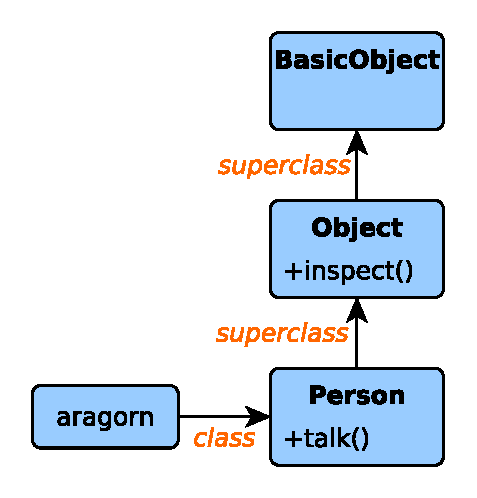
\includegraphics[scale=0.55]{diagrams/object_lookup_path.pdf}
\end{column}

\end{columns}

\end{frame}





\begin{frame}[fragile]\frametitle{Method lookup path: class object}

\begin{columns}[c] 

\begin{column}{7.4cm}

\begin{itemize}
\item A class is also an object!
\end{itemize}

\pause

\begin{lstlisting}[language=bash, escapechar={^}]
irb(main):005:0> aragorn = Person.new
=> #<Person:0x0000000285c3a0>
irb(main):006:0> aragorn.class
=> Person                           ^\pause^
irb(main):007:0> Person.class
=> Class                            ^\pause^
irb(main):008:0> Class.superclass
=> Module                           ^\pause^
irb(main):009:0> Module.superclass
=> Object                           ^\pause^
irb(main):010:0> Object.superclass 
=> BasicObject
\end{lstlisting}

\end{column}
\pause

\begin{column}{3.9cm}
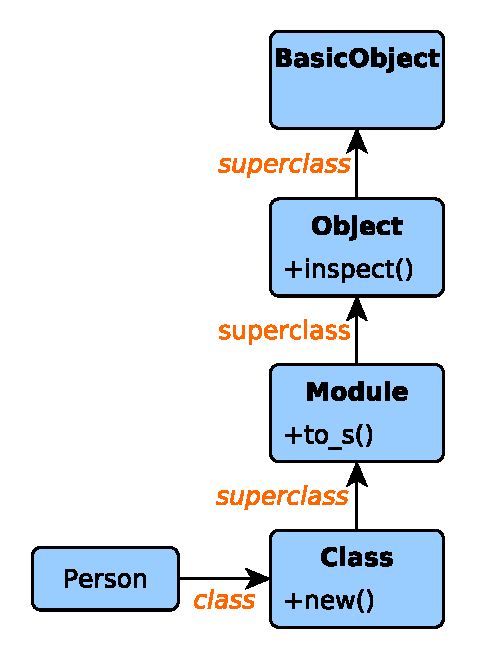
\includegraphics[scale=0.55]{diagrams/class_object_lookup_path.pdf}
\end{column}

\end{columns}

\end{frame}




\begin{frame}[fragile]\frametitle{Singleton Methods}

\begin{itemize}
\item A class defines the behaviour of their instances
\item Behaviour of person instances is placed in the Person class
\item Ruby allows unique behaviour to individual objects!
\end{itemize}

\pause
\lstinputlisting[language=ruby]{code/singleton_methods.rb}

\end{frame}




\begin{frame}[fragile]\frametitle{Eigenclasses (singleton classes, metaclasses, ghost classes)}

\begin{columns}[c] 

\begin{column}{5.5cm}
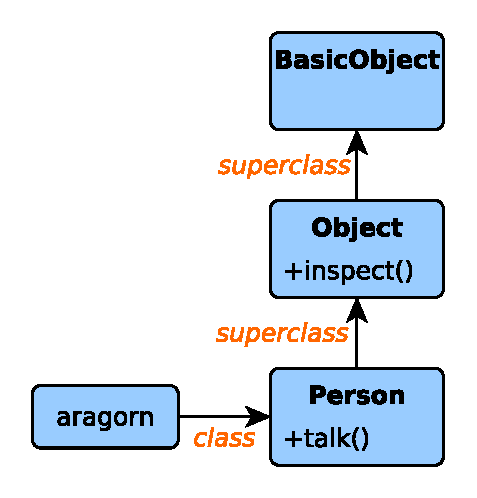
\includegraphics[scale=0.55]{diagrams/object_lookup_path.pdf}

\begin{itemize}
\item \alt<1>{Where is \texttt{aka}?}{There it is!}
\end{itemize}
\end{column}

\pause

\begin{column}{5.5cm}
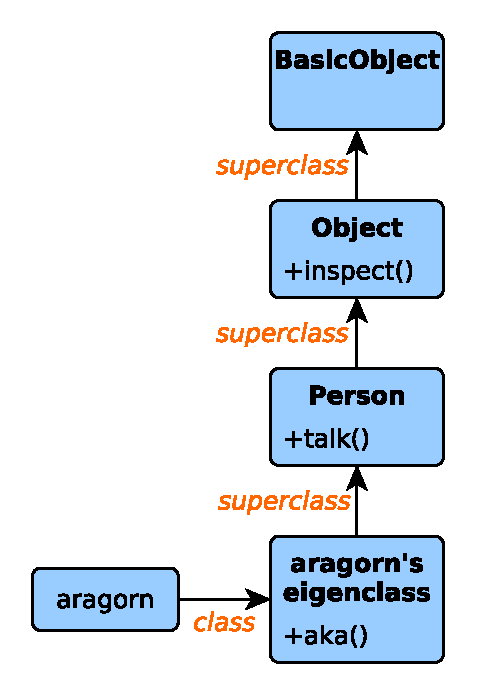
\includegraphics[scale=0.55]{diagrams/object_lookup_path2.pdf}
\end{column}

\end{columns}

\end{frame}




\begin{frame}[fragile]\frametitle{Eigenclasses and the \texttt{class <<} syntax}

\begin{columns}[c] 

\begin{column}{5.5cm}

\begin{itemize}
\item "one's very own" class
\item anonymous class
\item<3-> The \texttt{class <<} syntax opens the eigenclass of whatever object you pass to it
\end{itemize}

\end{column}

\pause

\begin{column}{5.5cm}

\lstinputlisting[language=ruby, firstline=4, lastline=6]{code/singleton_methods.rb}

\pause

\begin{lstlisting}[language=ruby, escapechar={^}]
class << aragorn
  def aka
    "Strider"
  end
end
\end{lstlisting}

\end{column}

\end{columns}

\end{frame}





\begin{frame}[fragile]\frametitle{Class Methods, revisited}

\begin{itemize}
\item classes are also objects, so
\begin{itemize}
\item ...they can have singleton methods 
\end{itemize}   \pause
\item In fact, what we call class methods are singleton methods for classes!
\end{itemize}

\pause

\begin{columns}[c] 

\begin{column}{5.5cm}

\begin{lstlisting}[language=ruby, escapechar={^}]
def Person.closest_dna
  "chimpanzee"
end
\end{lstlisting}
\pause
\begin{lstlisting}[language=ruby, escapechar={^}]
class Person
  def self.closest_dna
    "chimpanzee"
  end
end
\end{lstlisting}


\end{column}

\pause

\begin{column}{5.5cm}

\begin{lstlisting}[language=ruby, escapechar={^}]
class << Person
  def closest_dna
    "chimpanzee"
  end
end
\end{lstlisting}
\pause
\begin{lstlisting}[language=ruby, escapechar={^}]
class Person
  class << self
    def closest_dna
      "chimpanzee"
    end
  end
end
\end{lstlisting}

\end{column}

\end{columns}

\end{frame}




\begin{frame}\frametitle{Complete lookup path}
\begin{center}
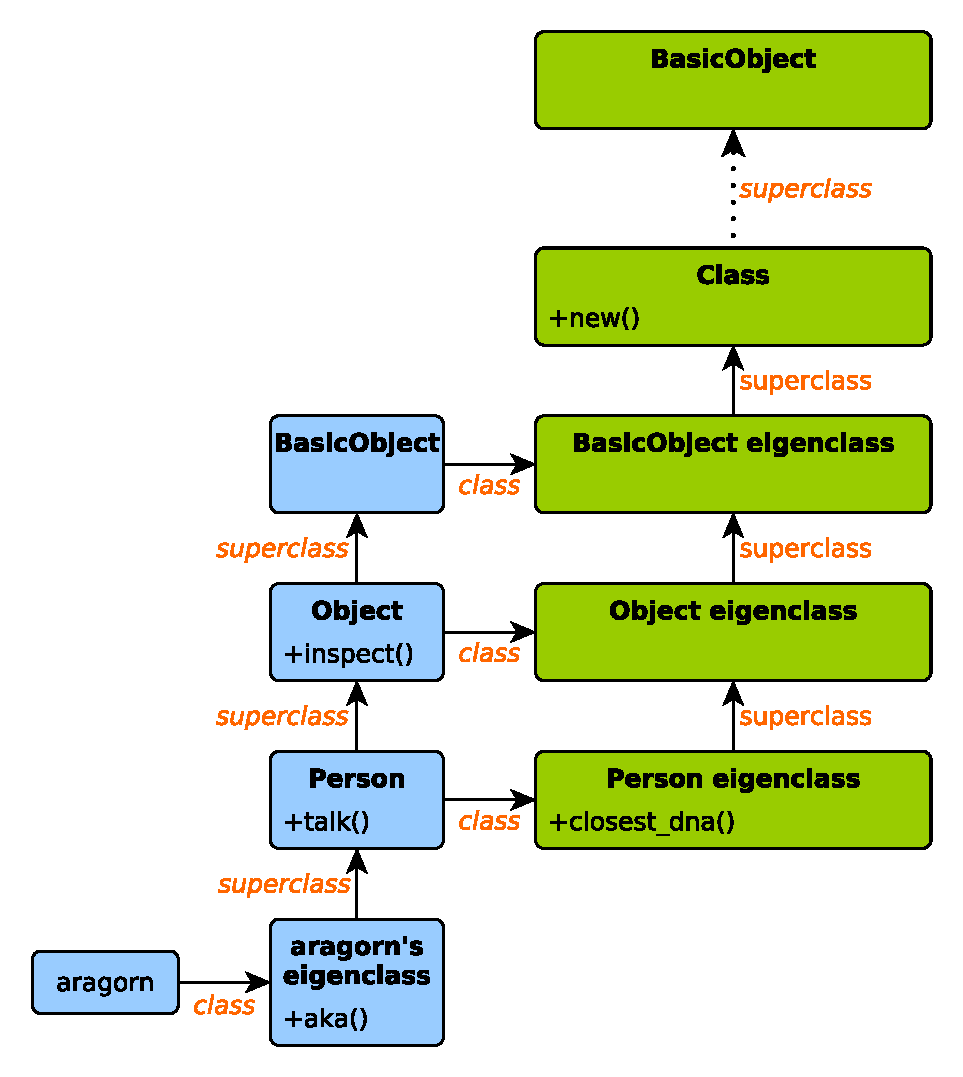
\includegraphics[scale=0.42]{diagrams/complete_lookup_path.pdf}
\end{center}
\end{frame}




\subsection{Modules}
\begin{frame}[fragile]\frametitle{Modules}

\begin{itemize}

\item A way of grouping together methods, classes and constants

\begin{itemize}
\item namespaces
\end{itemize}

\end{itemize}

\pause

\begin{columns}[c]

\begin{column}{5.3cm}
\begin{lstlisting}[language=bash, escapechar={^}]
irb:001> Math.sqrt(9)
 => 3.0                  ^\pause^
irb:002> Math::PI
 => 3.141592653589793    ^\pause^
irb:003> include Math
 => Object               ^\pause^
irb:004> sqrt(5)
 => 2.23606797749979     ^\pause^
irb:005> PI
 => 3.141592653589793 
\end{lstlisting}
\end{column}

\pause

\begin{column}{5.3cm}
\lstinputlisting[language=ruby]{code/module_trig.rb}
\end{column}

\end{columns}

\end{frame}





\begin{frame}[fragile]\frametitle{Modules, cont.}

\begin{itemize}

\item A way of adding extra functionality to classes

\begin{itemize}
\item mixins
\end{itemize}

\end{itemize}

\pause

\begin{columns}[c]

\begin{column}{5.4cm}
\lstinputlisting[language=ruby]{code/my_logger.rb}
\end{column}

\pause

\begin{column}{5.4cm}
\lstinputlisting[language=ruby]{code/person_mixins.rb}
\end{column}

\end{columns}

\end{frame}





\begin{frame}[fragile]\frametitle{Mixins, another example}

\begin{itemize}

\item Even more useful when mixin code interacts with class

\begin{itemize}
\item \texttt{Comparable} provides \texttt{<, <=, ==, >=, >, between?}
\item \texttt{Comparable} assumes class implements \texttt{<=>}
\end{itemize}

\end{itemize}

\pause

\begin{columns}[c]

\begin{column}{5.4cm}
\lstinputlisting[language=ruby, lastline=15]{code/person_comparable.rb}
\end{column}

\pause

\begin{column}{5.4cm}
\lstinputlisting[language=ruby, firstline=17, firstnumber=17]{code/person_comparable.rb}
\end{column}

\end{columns}

\end{frame}






\subsection{Files}
\begin{frame}[fragile]\frametitle{Files}

\begin{itemize}

\item Organise code into multiple files

\begin{itemize}
\item \texttt{load}
\item \texttt{require}
\item \texttt{require\_relative}
\end{itemize}

\end{itemize}

\pause

\begin{itemize}

\item Load path

\begin{itemize}
\item \texttt{\$LOAD\_PATH} or \texttt{\$:}
\end{itemize}

\end{itemize}


\end{frame}
%http://ruby.about.com/od/rubysbasicfeatures/ss/Load-Vs-Require.htm




\section{System Interaction} 
\begin{frame}\frametitle{System Interaction} 
\begin{itemize}
\item File System
\item Arguments
\item Environment
\item Shebang (hashbang)
\item Ruby Command Line
\end{itemize}
\end{frame}






\subsection{File System}
\begin{frame}[fragile]\frametitle{\texttt{File}}

\begin{columns}[c]

\begin{column}{7cm}

\begin{lstlisting}[language=ruby, escapechar={^}]
f = File.new("filename", "r")
f.each_line { |l| puts l }
f.close
\end{lstlisting}

\pause

\begin{lstlisting}[language=ruby, escapechar={^}]
File.open("filename", "r") do |f|
   f.each_line { |l| puts l }
end
\end{lstlisting}

\pause

\begin{lstlisting}[language=ruby, escapechar={^}]
IO.foreach("filename") { |l| puts l }
\end{lstlisting}

\end{column}

\pause

\begin{column}{4cm}
\begin{itemize}

\item \texttt{File}

\begin{itemize}
\item \texttt{.size}
\item \texttt{.exists?}
\item \texttt{.directory?}
\item \texttt{.writable?}
\item \texttt{.delete}
\item \texttt{.rename}
\item \texttt{.chown}
\item \texttt{.ctime}

\end{itemize}

\end{itemize}
\end{column}

\end{columns}

\end{frame}




\begin{frame}[fragile]\frametitle{\texttt{Dir}}

\begin{columns}[c]

\begin{column}{7cm}

\begin{lstlisting}[language=ruby, escapechar={^}]
Dir.foreach("/usr/bin") do |entry|
   puts entry
end
\end{lstlisting}

\pause

\begin{lstlisting}[language=ruby, escapechar={^}]
Dir.entries("/usr/bin").join(' ')
\end{lstlisting}

\pause

\begin{lstlisting}[language=ruby, escapechar={^}]
Dir["/usr/bin/*"]
\end{lstlisting}

\end{column}

\pause

\begin{column}{4cm}
\begin{itemize}

\item \texttt{Dir}

\begin{itemize}
\item \texttt{.chdir}
\item \texttt{.mkdir}
\item \texttt{.pwd}

\end{itemize}

\end{itemize}
\end{column}

\end{columns}

\end{frame}







\subsection{Arguments}
\begin{frame}[fragile]\frametitle{Arguments}

\begin{itemize}

\item Command-line arguments

\begin{itemize}
\item \texttt{ARGV} array
\item \texttt{ARGV.each \{ |a| puts a \}}
\end{itemize}

\item Check \texttt{optparse} from standard library

\end{itemize}

\end{frame}




\subsection{Environment}
\begin{frame}[fragile]\frametitle{Environment}

\begin{itemize}

\item Reading OS's environment variables

\begin{itemize}
\item \texttt{ENV} hash
\item \texttt{ENV.each \{ |k,v| puts "\#\{k\}=\#\{v\}" \} }
\end{itemize}

\end{itemize}

\end{frame}




\subsection{Shebang (hashbang)}
\begin{frame}[fragile]\frametitle{Shebang (hashbang)}
\begin{lstlisting}[language=ruby, escapechar={^}]
#!/usr/bin/env ruby

puts "Hello World!"
\end{lstlisting}
\pause
\begin{lstlisting}[language=bash, escapechar={^}]
$ chmod 755 file.rb
$ ./file.rb
Hello World
$
\end{lstlisting}
\end{frame}





\subsection{Ruby Command Line}
\begin{frame}[fragile]\frametitle{Ruby Command Line}

\begin{itemize}

\item Command line options

\begin{itemize}
\item \texttt{-v}
\pause
\item \texttt{-e}
\begin{itemize}
\item \lstinline!$ ruby -e 'puts "Hi"'!
\end{itemize}
\pause
\item \texttt{-n}
\begin{itemize}
\item \texttt{while gets; ... end}
\item \lstinline!$ echo -e "foo\nbar" | ruby -ne 'puts $_'!
\end{itemize}
\pause
\item \texttt{-p}
\begin{itemize}
\item \texttt{operates on \texttt{\$\_}} and writes it at every iteration
\item \lstinline!$ echo -e "foo\nbar" | ruby -pe 'chomp'!
\end{itemize}

\end{itemize}

\end{itemize}

\end{frame}






\section{Miscellaneous} 
\begin{frame}\frametitle{Miscellaneous} 
\begin{itemize}
\item Regular Expressions
\item Web Services
\item Concurrency: a bird's eye view
\item Metaprogramming: a bird's eye view
\end{itemize}
\end{frame}




\subsection{Regular Expressions}
\begin{frame}[fragile]\frametitle{Regular Expressions}

\begin{itemize}

\item A pattern that can be matched against a string

\begin{itemize}
\item \texttt{r = Regexp.new("pattern")}
\pause
\item \texttt{r = /pattern/}
\pause
\item \texttt{r = \%r\{pattern\}}
\pause
\item Operators: \texttt{=\~} and \texttt{!\~}
\end{itemize}

\end{itemize}

\pause

\begin{lstlisting}[language=ruby, escapechar={^}]
/lo/ =~ "hello"                         # => 3     ^\pause^
"hello" =~ /lo/                         # => 3     ^\pause^
"hello" =~ /hi/                         # => nil   ^\pause^
m = /ll/.match("hello")                 # => #<MatchData "ll"> ^\pause^
"#{m.pre_match}->#{m[0]}<-#{m.post_match}" 
# => "he->ll<-o" ^\pause^

if "hello" =~ /hi/
  # ..
end
\end{lstlisting}

\end{frame}




\begin{frame}[fragile]\frametitle{Regular Expressions, cont.}

\begin{itemize}

\item All characters match themselves except:

\begin{itemize}
\item \lstinline!. | ( ) [ ] { } + \ ^ $ * ?!
\end{itemize}

\end{itemize}

\pause

\begin{lstlisting}[language=ruby, escapechar={!}]
"hello" =~ /^el/                        # => nil !\pause!
"hello " =~ /lo$/                       # => nil !\pause!
"hello " =~ /[aeiou]/                   # => 1   !\pause!
"hello world" =~ /\s/                   # => 5   !\pause!
"hello world" =~ /\s[[:digit:]]/        # => nil !\pause!
"bat bit bot bet" =~ /(b.t )*/          # => 0   !\pause!
print $~                                # bat bit bot  => nil !\pause!
"bat bit bot bet" =~ /(b.t ){2}/        # => 0   !\pause!
print $~                                # bat bit => nil  !\pause!
"mississipi" =~ /(...)\1/i              # => 1   !\pause!
print $~                                # ississ => nil 
\end{lstlisting}

\end{frame}





\subsection{Web Services}
\begin{frame}[fragile]\frametitle{REST (\texttt{rest-client})}
\lstinputlisting[language=ruby]{code/rest_example.rb}
\end{frame}



\begin{frame}[fragile]\frametitle{SOA/SOAP (\texttt{savon} -- v2)}
\lstinputlisting[language=ruby]{code/soap_example.rb}
\end{frame}





\subsection{Concurrency: a bird's eye view}
\begin{frame}\frametitle{Concurrency: a bird's eye view}

\begin{itemize}[<+->]

\item Processes

\item Threads
\begin{itemize}

\item green threads (v1.8)
\item native threads (v1.9)
\begin{itemize}
\item GIL: data modified only by one thread at a time
\item ...but another thread could do I/O
\end{itemize}
\item JRuby, IronRuby, MacRuby, Rubinius, ...
\end{itemize}

\item Fibers
\begin{itemize}
\item \emph{lightweight} threads
\item ...but controlled by the developer
\end{itemize}

\end{itemize}

\end{frame}
%http://merbist.com/2011/02/22/concurrency-in-ruby-explained/



\subsection{Metaprogramming: a bird's eye view} 
\begin{frame}\frametitle{Metaprogramming: a bird's eye view} 
\begin{itemize}[<+->]

\item DSLs: writing code that writes code

\item Classes (and other language constructs) definition
\begin{itemize}
\item C, Pascal, ...
\item ...at compile time
\item Java, ...
\item ...at compile time and provides read access at runtime
\item Ruby
\item ...at compile time and provides read/write access at runtime
\end{itemize}

\end{itemize}
\end{frame}




\end{document}